\section{Experiments}
\label{sec:exp}

\paragraph{Overview.} We organize the evaluation as a single causal chain. \Cref{sec:rq1} showed the built-in confidence is uneven and
collapses out-of-distribution; this motivates a perturbation estimator. \Cref{sec:exp-main} shows
that estimator significantly beats the built-in confidence on $9$ of $12$ cells, \emph{including the
out-of-distribution set for all three architectures}, and that the wins are \emph{predicted} by where
the confidence was mis-calibrated. \Cref{sec:exp-arch} shows the win holds across all three
architectures and that the architecture governs \emph{which} perturbation carries the signal.
\Cref{sec:probe} shows the signal is \emph{epistemic}---it beats a probe trained on the model's own
features, so it cannot be a static property of one forward pass. \Cref{sec:exp-fusion} converts the
better ranking into a concrete geometry payoff (multi-view fusion), and \Cref{sec:exp-neg} reports
where the method does \emph{not} help.

\subsection{Protocol, baselines, and cost}
\label{sec:exp-protocol}

\paragraph{Protocol.} We evaluate on \textbf{7-Scenes} (RGB-D, indoor, in-distribution), \textbf{DTU}
(structured-light, object-centric, mm-scale, in-distribution), \textbf{BlendedMVS} (rendered MVS; a
standard \emph{training} corpus for these models, hence an in-distribution \emph{control}), and
\textbf{ETH3D} (laser, wide-baseline DSLR, \emph{out-of-distribution})---a full $3{\times}4$
model$\times$dataset grid. Unless noted we use $5$ views and $N{=}5$ samples in bfloat16;
perturbation inputs are capped to $\le 1024$\,px on the longest side (this affects only ETH3D's native
$6198{\times}4129$ source; the models resize every input to ${\sim}518$\,px internally, so the cap is
near-lossless). Every number is the mean over \textbf{3 seeds}, and significance is a \textbf{paired
Wilcoxon} signed-rank test over view-sets (\Cref{sec:primer-metrics}). Each plot shows the
\emph{oracle} (error-sorted) floor and the \emph{random} reference. All runs fit on one RTX 5060 Ti
(16\,GB).

\paragraph{Baselines.} Beyond the built-in confidence, we compare against \emph{random} and
\emph{oracle} bounds on every plot, a \emph{trained probe} on the model's frozen features
(\Cref{sec:probe}), and an \emph{MC} estimator (\Cref{tab:rq2}): because the released checkpoints
expose no dropout, we approximate Monte-Carlo sampling at the only stochastic surface available
without retraining---the \emph{input}---by adding zero-mean Gaussian noise to the images (standard
deviation ${\approx}1.5\%$ of the intensity range) and aggregating exactly as \trustr\ does. It is a
deliberately simple, fixed-magnitude analogue of MC-dropout~\cite{mcdropout}: undirected input noise
\emph{without} the geometry-preserving structure and gauge alignment that distinguish \trustr.
Weight-perturbation deep ensembles~\cite{ensembles} need multiple trained models and are out of scope
for frozen, inference-only deployment.

\paragraph{Cost.} A full \trustr\ map is $N{=}5$ passes per family; per-model wall-clock and memory
are in \Cref{tab:runtime} ($11\text{--}15$\,s, $\le 9$\,GB). $N{=}5$ is a knee, not a floor: $N{=}3$
already recovers $93\%$ of the accuracy gain at $0.57\times$ the cost ($5.2$ versus $9.1$\,s;
\Cref{tab:latencyn}), so latency-critical users can trade a little accuracy for speed.

\begin{table}[tb]
  \centering\small
  \adjustbox{max width=\columnwidth}{\input{tables/tab_runtime}}
  \caption{\textbf{Cost} on the 16\,GB GPU: one frozen forward and a full \trustr\ estimate
  ($N{=}5$, two families).}
  \label{tab:runtime}
\end{table}

\begin{table}[tb]
  \centering\small
  \adjustbox{max width=\columnwidth}{\input{tables/tab_latency_n}}
  \caption{\textbf{Accuracy vs.\ cost} (\vggt/7-Scenes): \trustr\ wall-clock and \ause\ at
  $N{=}2/3/5$; $N{=}3$ recovers $93\%$ of the $N{=}5$ gain over the built-in confidence at
  $\sim$half the cost.}
  \label{tab:latencyn}
\end{table}

\begin{figure}[tb]
  \centering
  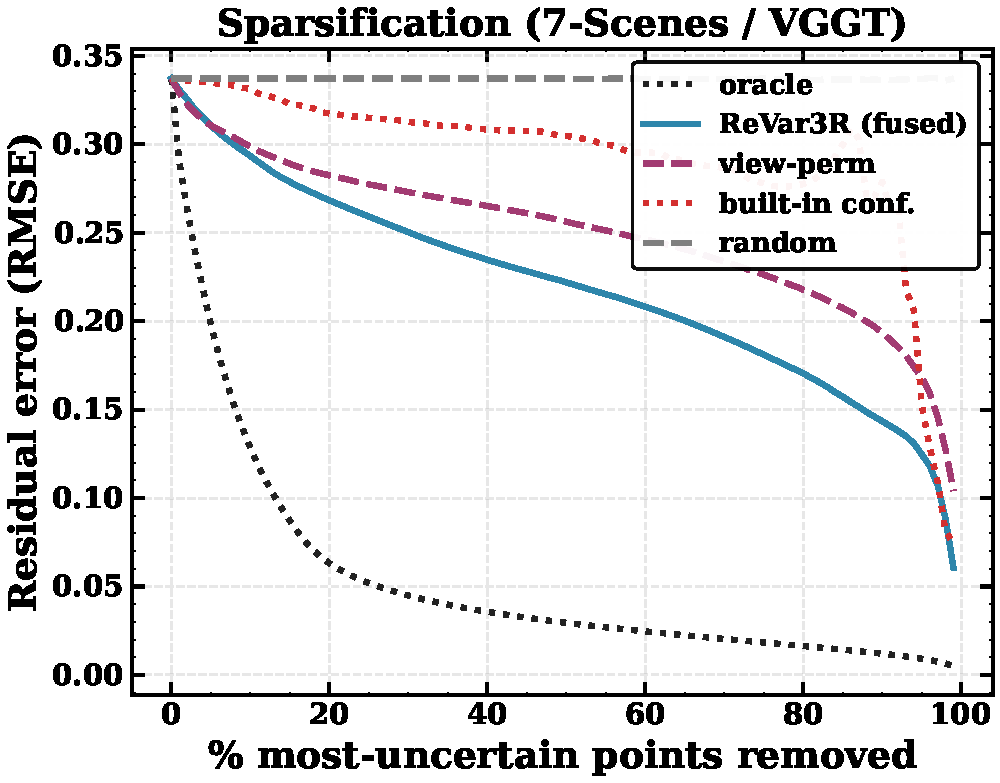
\includegraphics[width=\linewidth]{rq2_sparsification_clean_vggt_sevenscenes.pdf}
  \caption{\textbf{Sparsification} (\vggt/7-Scenes). \trustr's residual-error drop tracks the
  \emph{oracle}; the built-in confidence barely beats \emph{random}. The gap between the curves is the
  \ause.}
  \label{fig:spars}
\end{figure}

\subsection{Main result: \trustr\ beats the built-in confidence}
\label{sec:exp-main}

Throughout, \trustr\ denotes a single headline estimator: the held-out, inverse-\ause-weighted rank
fusion of the two perturbation families \emph{together with} the model's own built-in confidence
(\Cref{sec:method}); the perturbation-only and equal-weight variants are reported beside it
(\Cref{sec:ablations}). \Cref{tab:rq2}, \Cref{fig:spars}, and \Cref{fig:cross} report the headline.
Across the full $3{\times}4{=}12$ grid, \trustr\ significantly reduces \ause\ in \textbf{9 of 12}
cells (by $3\text{--}36\%$; $p$ from $3{\times}10^{-2}$ to $9{\times}10^{-10}$), lifting Spearman
from $\le{+}0.07$ to as high as $+0.49$, and it \emph{restores the sign} of the correlation where it
was negative (\vggt/BlendedMVS $-0.12\to+0.43$, \mastr/DTU $-0.10\to+0.23$).

\paragraph{The headline is the out-of-distribution result.} On ETH3D, where the built-in confidence
flat-lines (Spearman $\approx 0$ for all three models), \trustr\ wins for \emph{every} architecture
($-3$ to $-10\%$, $p\le 6{\times}10^{-3}$): a training-free signal survives the very shift that breaks
the model's own confidence. We are careful about what carries this. Out-of-distribution it is the
\emph{perturbation} signal, not the fusion machinery: the simplest input-noise baseline (MC) already
matches or beats the built-in-augmented fusion on ETH3D, and a perturbation-only fusion is marginally
stronger there (the held-out fusion pays a small OOD cost for admitting the correlation-collapsed
built-in confidence as a candidate family; \Cref{sec:abl-fusion}). Both still clear the built-in
confidence---the deployed baseline---which is the claim we make.

\paragraph{The wins are predicted by mis-calibration---and so are the non-wins.} The three non-wins
are exactly the BlendedMVS column: the models' own training corpus, where the built-in confidence is
\emph{already} well-calibrated and \trustr\ correctly adds little. This coupling is stronger and more
honest than blanket superiority---indeed a perfect $12/12$ would be \emph{suspicious}, implying the
method ``improves'' even where the confidence is already good, which would suggest it is fitting
noise. (On BlendedMVS a large pooled $\Delta$ and the paired $p$ can look discordant---\vggt\ shows a
$-48\%$ pooled reduction yet $p{=}0.19$---because this rendered corpus mixes heterogeneous source
scans: the built-in confidence is locally sensible but globally mis-scaled, so its \emph{per-set}
\ause\ ($0.38$ for \vggt) is far below its \emph{pooled} $0.78$, and the per-set Wilcoxon we report
correctly factors that cross-scene scaling out; \Cref{sec:primer-metrics}.) \Cref{fig:qual} shows the
maps: \trustr's uncertainty mirrors true-error structure where the built-in confidence does not.

\begin{table*}[tb]
  \centering\small
  \adjustbox{max width=\textwidth}{\input{tables/tab2_rq2}}
  \caption{\textbf{Main result} (\ause\dn, mean over 3 seeds). \trustr\ has lower \ause\ in $10/12$
  cells ($\Delta<0$) and a \textbf{significant} win (paired-Wilcoxon $p<0.05$ \emph{and} lower \ause;
  \best{bold}) in \textbf{9 of 12}, \emph{including OOD for all three models}. The three non-wins are
  the BlendedMVS column---the models' own training corpus, where the built-in confidence is already
  well-calibrated.}
  \label{tab:rq2}
\end{table*}

\begin{figure}[tb]
  \centering
  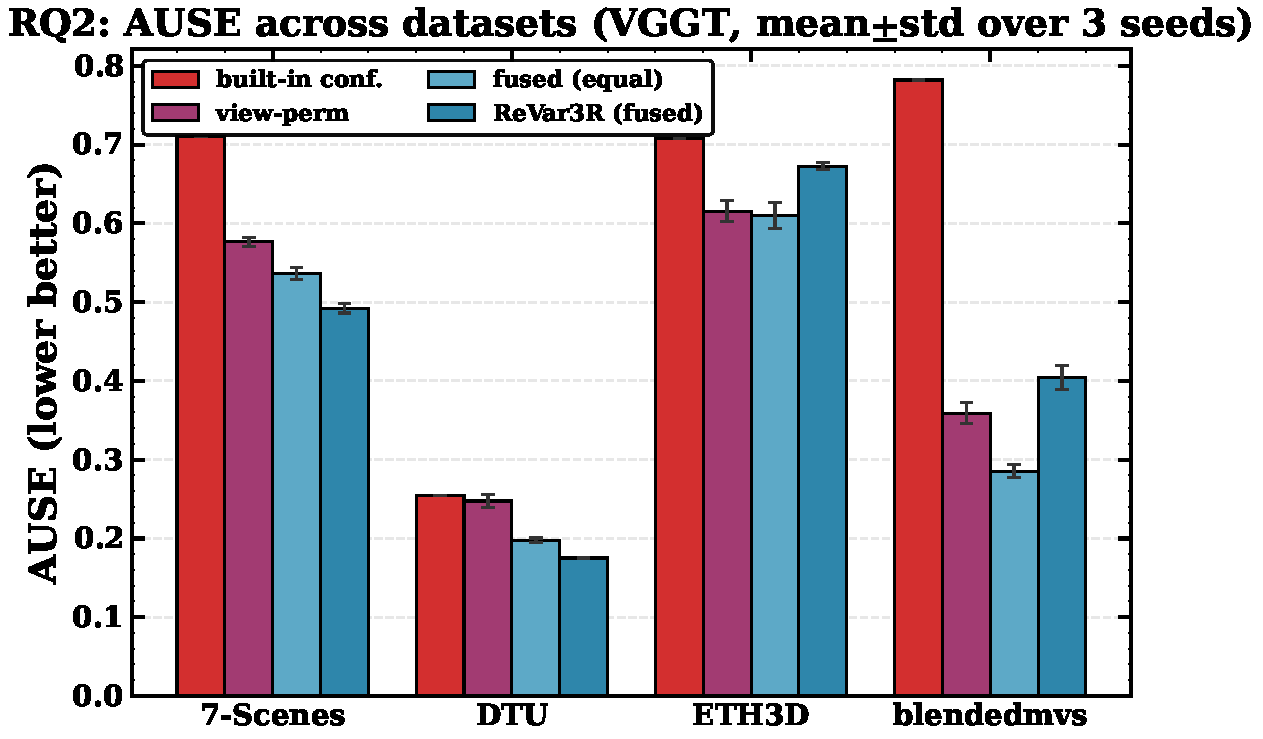
\includegraphics[width=\linewidth]{rq2_cross_dataset.pdf}
  \caption{\textbf{Cross-dataset \ause} (\vggt, mean$\pm$std over 3 seeds). The built-in confidence
  (red) is the weakest signal on all four datasets and \trustr\ (held-out weighted fusion) the
  strongest; the margin is largest on BlendedMVS and OOD ETH3D, where the built-in confidence is
  mis-calibrated ($\rho<0$ and $\approx 0$).}
  \label{fig:cross}
\end{figure}

\begin{figure*}[tbp]
  \centering
  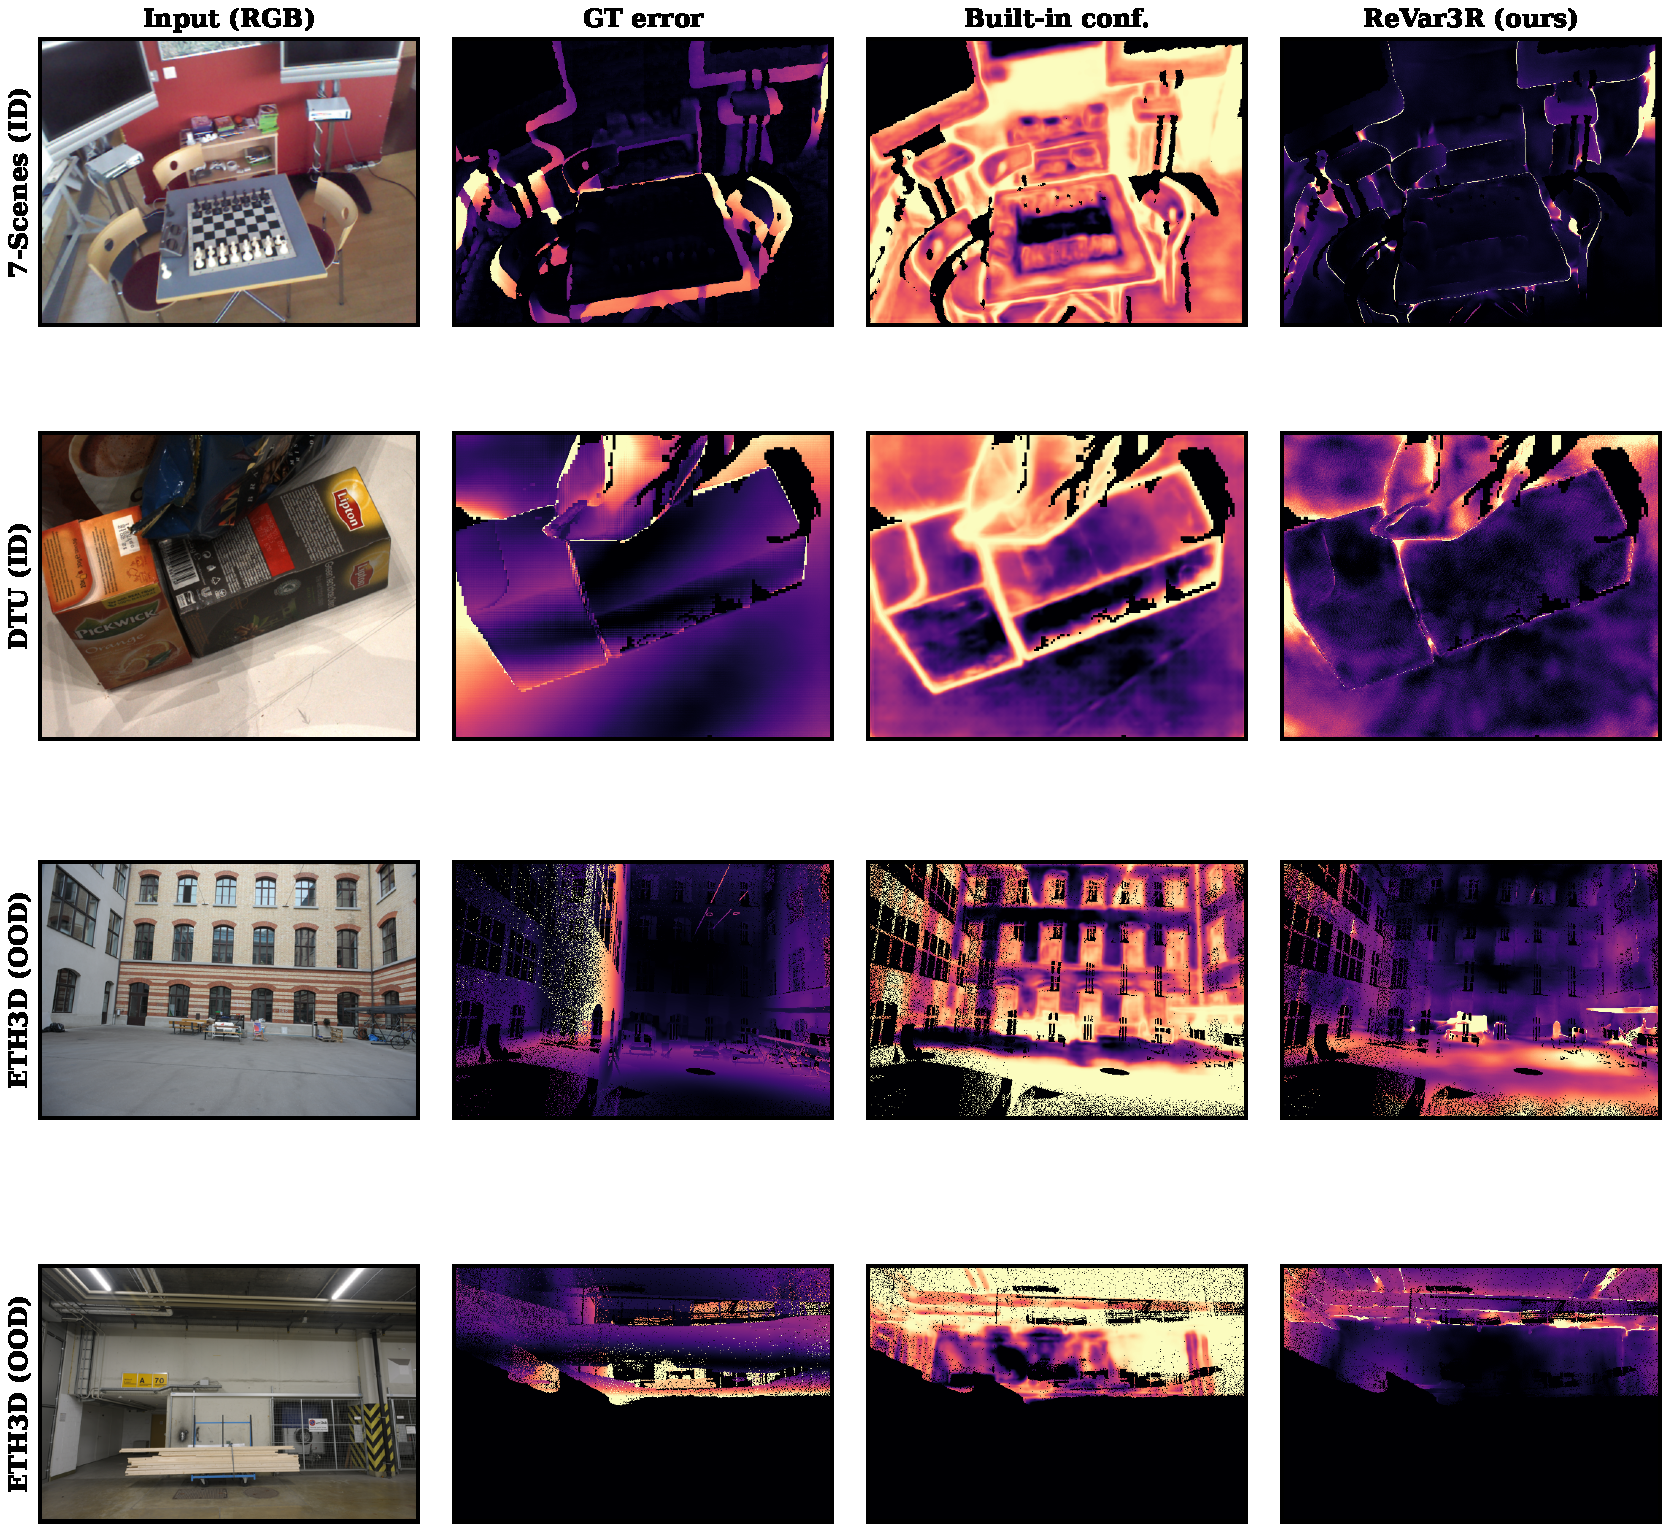
\includegraphics[width=0.92\linewidth]{qualitative.pdf}
  \caption{\textbf{Qualitative} (\vggt). For a reference view: input, GT error, built-in confidence
  (as uncertainty), and \trustr. \trustr\ highlights the genuinely-erroneous regions (object
  boundaries, textureless and far-depth areas); the built-in confidence is diffuse and, OOD,
  uncorrelated. Brighter $=$ more uncertain.}
  \label{fig:qual}
\end{figure*}

\subsection{The win holds across architectures, which govern the signal}
\label{sec:exp-arch}

\Cref{fig:bymodel} and \Cref{tab:rq2} show \trustr\ beats the built-in confidence on all three
architectures on 7-Scenes and ETH3D---the reference-dependent \vggt\ and \mastr\ ($-36\%$) and the
permutation-equivariant \pii\ ($0.509\to0.359$, $-29\%$ on 7-Scenes; $-10\%$ OOD). The gains are
architecture-agnostic \emph{where the built-in confidence is mis-calibrated}; on \pii's
already-well-calibrated BlendedMVS it correctly does not improve.

Crucially, the architecture governs \emph{which} perturbation carries the signal, exactly as the
gauge analysis (\Cref{sec:primer-gauge}) predicts. For the reference-dependent \vggt/\mastr,
view-permutation is the strongest single perturbation; for the equivariant \pii, where re-ordering is
inert by construction, the signal comes from photometric jitter and view-\emph{subset}, and the
held-out weighting drives the inert shuffle's weight to $\approx 0$ automatically. The
\emph{fitted fusion weight}---high on the view-perm family for \vggt/\mastr, near zero for
\pii---reads this architectural fact out cleanly, with no special-casing in the pipeline
(full per-signal breakdown in \Cref{sec:abl-fusion}).

\begin{figure}[tb]
  \centering
  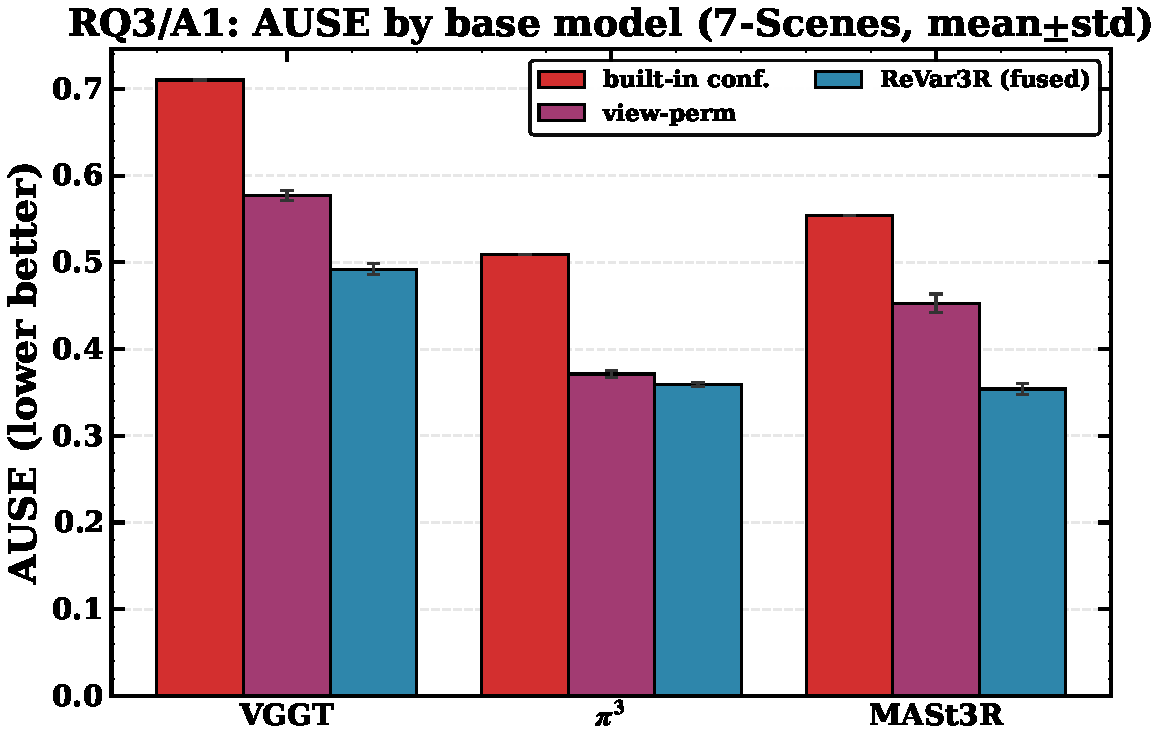
\includegraphics[width=\linewidth]{rq3_by_model.pdf}
  \caption{\textbf{By base model} (7-Scenes). \trustr\ beats the built-in confidence on \vggt, \pii,
  and \mastr.}
  \label{fig:bymodel}
\end{figure}

\subsection{The signal is epistemic, not in the features}
\label{sec:probe}

If \trustr\ merely re-discovered information already present in one forward pass, a model trained to
read that information should match it. We test this directly. We train a small MLP probe on the
model's \emph{frozen} features (final-aggregator patch tokens, bilinearly sampled to pixels) to
regress per-point error, on held-out scenes with a leakage-free 2-fold split---the strongest
\emph{trained} reference. \Cref{tab:probe} shows \trustr\ \emph{matches or beats this trained probe on
\ause\ on every dataset}. On 7-Scenes the probe cannot even beat the built-in confidence
($0.79$ versus $0.70$)---the error signal is \emph{not} linearly decodable from a single forward
pass---yet \trustr\ reaches Spearman $+0.29$ where the probe reaches $+0.09$.

The interpretation is mechanistic: the usable signal is \emph{consistent with epistemic
input-sensitivity}, visible only when the model is re-run under perturbations, not a static feature
decodable in one pass. This is the empirical core of the paper's conceptual claim
(\Cref{sec:method-idea}). We are careful not to overclaim: on DTU the probe \emph{does} decode real
signal ($\rho{=}0.56$) and \trustr\ still wins the sparsification \ause, but the probe is a
\emph{reasonable}, not maximal, trained reference (one backbone, a single feature tap, a small MLP);
a stronger decoder---spatial context, multi-layer features---might recover more. This is therefore
\emph{evidence for} the epistemic interpretation, not a proof of an upper bound.

\begin{table}[tb]
  \centering\small
  \adjustbox{max width=\columnwidth}{\input{tables/tab3_probe}}
  \caption{\textbf{\trustr\ vs.\ a trained probe} on the model's frozen features (\ause\dn, Spearman).
  Training-free \trustr\ matches/beats the trained probe everywhere; on 7-Scenes the probe cannot
  beat the built-in confidence.}
  \label{tab:probe}
\end{table}

\subsection{Downstream utility: uncertainty-gated multi-view fusion}
\label{sec:exp-fusion}

A better ranking should translate into a better cloud. When the per-view point maps are fused into one
cloud and the least-trusted points are dropped, \trustr\ selects the wrong points far better than the
built-in confidence (\Cref{fig:fusion}, \Cref{tab:fusion}): at $10\%$ removed it is near-oracle
($0.029$ versus built-in $0.034$\,m on 7-Scenes; $4.10$ versus $4.81$\,mm on DTU), and on DTU it
preserves far more completeness---at $50\%$ removed, confidence-filtering destroys coverage
($20.4$\,mm) while \trustr\ keeps it intact ($9.7$\,mm). This is a concrete, geometry-level payoff for
the better ranking. We report it as an \emph{in-distribution} utility: on OOD ETH3D the fusion gain is
null on \emph{both} accuracy and completeness (all signals $\approx 0.90$\,m accuracy and
$\approx 2.3$\,m completeness at every removal fraction), which we state plainly rather than overclaim.

\begin{figure*}[tbp]
  \centering
  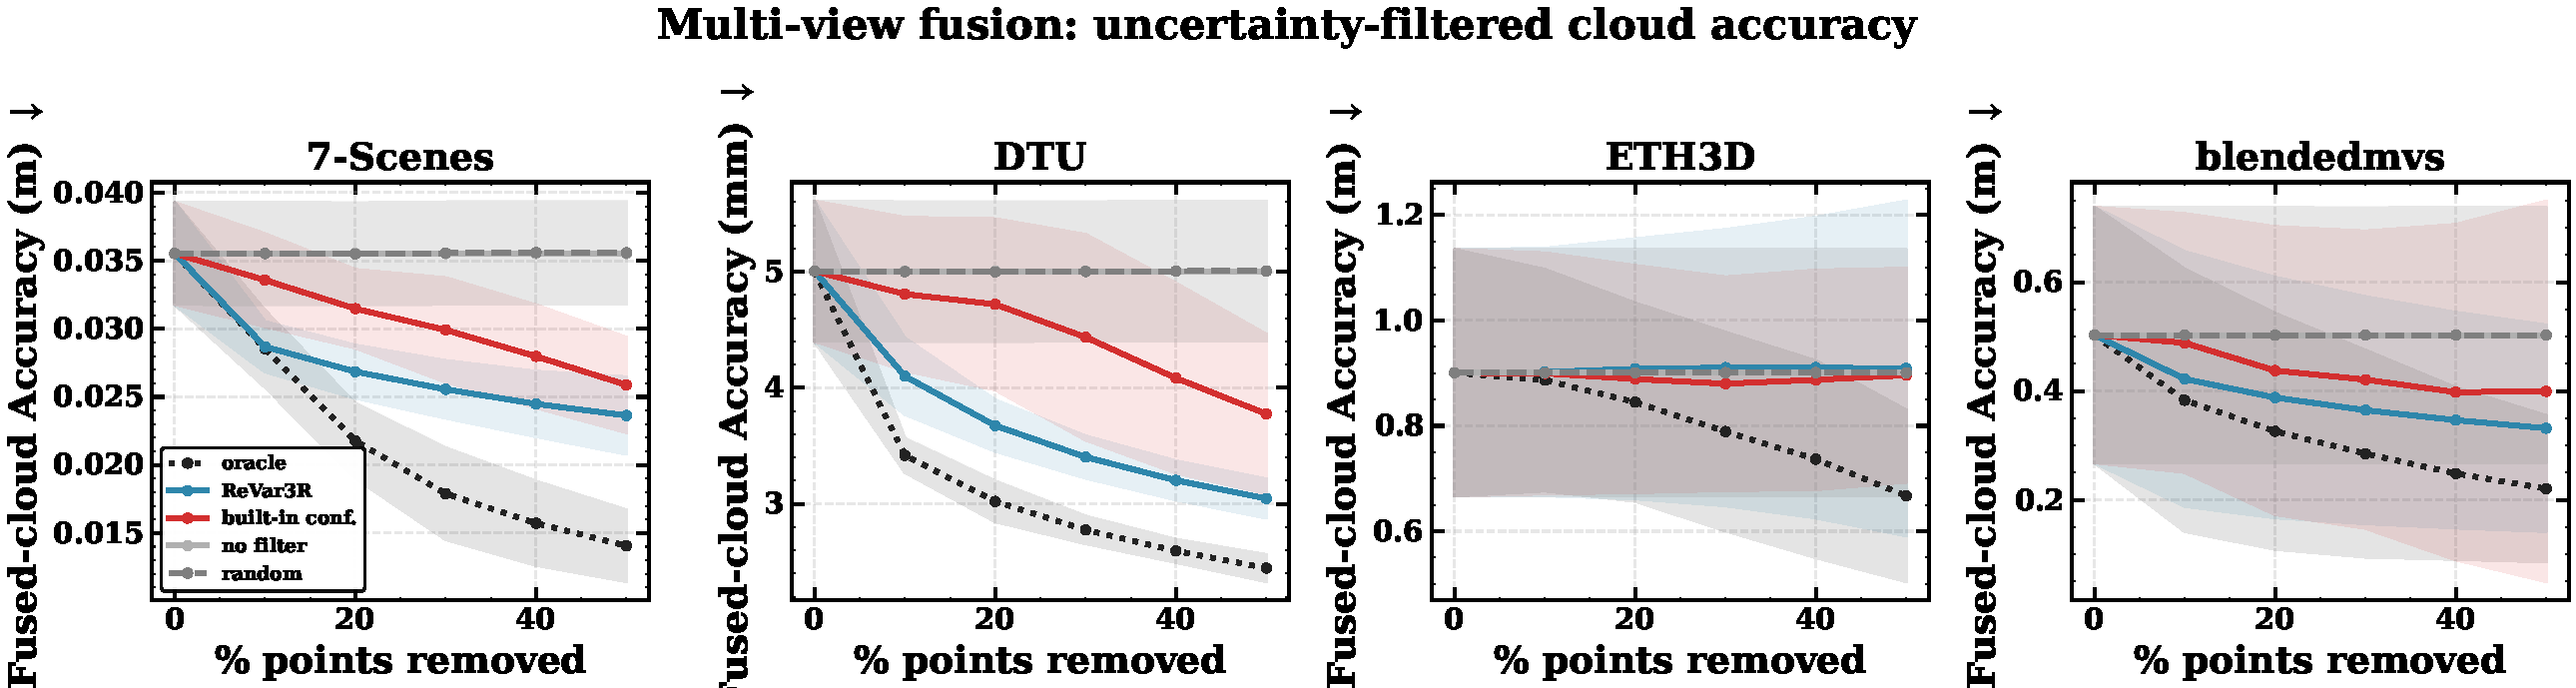
\includegraphics[width=0.96\linewidth]{fusion_accuracy_all.pdf}
  \caption{\textbf{Multi-view fusion.} Fused-cloud Accuracy vs.\ fraction of least-trusted points
  removed. \trustr\ (blue) tracks the oracle on 7-Scenes/DTU; OOD ETH3D shows no gain (stated
  honestly).}
  \label{fig:fusion}
\end{figure*}

\begin{table*}[tb]
  \centering\small
  \adjustbox{max width=\textwidth}{\input{tables/tab5_fusion}}
  \caption{\textbf{Fused-cloud quality} (lower is better). \trustr-filtered fusion is near-oracle and,
  on DTU, preserves much more completeness than confidence-filtering.}
  \label{tab:fusion}
\end{table*}

\subsection{Honest negatives}
\label{sec:exp-neg}

\paragraph{Novel-view synthesis (the null part of H4).} Using \trustr\ to filter 3D Gaussian-Splatting
initialization gives \emph{no} PSNR advantage (all signals within $\sim 0.4$\,dB; random competitive).
This is consistent with our thesis: NVS quality is dominated by appearance/aleatoric factors that the
long per-scene optimization absorbs, not the epistemic geometry uncertainty \trustr\ captures. We
therefore lead the downstream story with multi-view fusion, and report the NVS null plainly
(Appendix~\ref{app:negatives}).

\paragraph{A falsified hypothesis (H3).} We hypothesized that view-permutation disagreement would be a
\emph{stronger} signal for the reference-dependent \vggt\ than for the equivariant \pii. It is not:
relative to each model's built-in confidence, view-perm helps \pii\ at least as much (its gain comes
through leave-one-out \emph{subset} rather than shuffle). The architecture shapes the signal, but not
in the hypothesized direction; we report the characterization (\Cref{sec:exp-arch}), not the original
claim, and analyze the reversal in Appendix~\ref{app:negatives}. Reporting it is the point: a reliability
study that hid its own falsified prediction would undercut its own credibility.
